\chapter{Methods}
\label{chp:methods}

\begin{center}
    \textit{Here, the development process and methodologies are described in detail. This includes the design and implementation of the desktop application, the selection of tools and frameworks, and the approach to solving the problem.}
\end{center}

\section{Development Methodology}
\label{sec:development-methodology}

\subsection{Agile Approach}
\label{subsec:agile-approach}

\subsection{Sprint Planning}
\label{subsec:sprint-planning}

\subsection{Code Reviews}
\label{subsec:code-review}

\section{Software Design}
\label{sec:software-design}

\subsection{Design Process}
\label{subsec:design-process}

\subsubsection*{User-Centered Design}
\label{subsubsec:user-centered-design}

At the beginning of the design process, the group conducted wireframe testing with a diverse set of users. This included participants of varying age groups—from young to elderly—as well as both chess players and non-chess players. The goal was to evaluate whether users found the interface intuitive and whether the sizing and layout were appropriate across different demographics. \\

All participants were given the same context before starting the test: 

\begin{quote}
\textit{You are viewing a chess game between two companions you know. You visit the tournament organizer's website and come across this webpage.}
\end{quote}

Participants were then either given specific tasks to perform within the application or asked to explore freely, mimicking a real-world scenario. This approach aimed to identify how naturally users could navigate and understand the application without explicit instruction. \\

After completing their interaction with the application, participants filled out an anonymous feedback form. This encouraged honest, unfiltered responses, reducing the likelihood of social desirability bias. The form included questions such as:

\begin{itemize}
    \item \textit{On a scale from 1 to 5, how satisfied are you with the overall experience of the application?}
    \item \textit{On a scale from 1 to 5, how satisfied are you with the Tournament View page?}
    \item \textit{On a scale from 1 to 5, how satisfied are you with the Board View page?}
    \item \textit{Do you have any feedback, suggestions for improvement, or features you would like to see added?}
\end{itemize}

This process aligns with the principles discussed in \ref{subsubsec:usability-testing}, as outlined in Chapter~\ref{chp:theory}.


\subsection{Diagrams}
\label{subsec:diagrams}

\subsubsection*{Sequence Diagram}
\label{subsubsec:sequence-diagram}

\begin{figure}[h!]
    \centering
    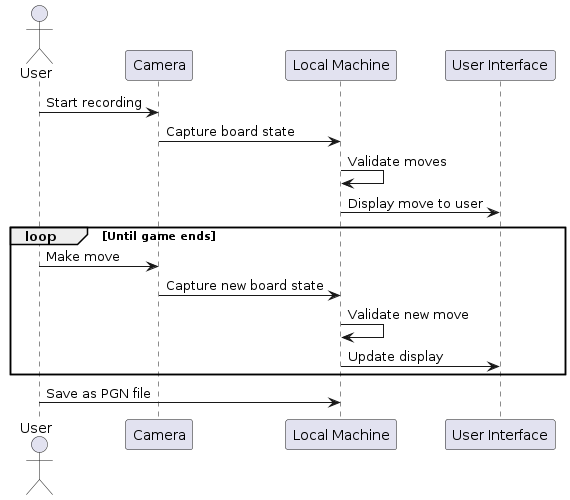
\includegraphics[width=0.75\linewidth]{figures/uml/sequence.png}
    \caption[Sequence Diagram]{Sequence Diagram}
    \label{fig:sequence}
\end{figure}

\subsubsection*{Activity Diagram}
\label{subsubsec:activity-diagram}

\begin{figure}[h!]
    \centering
    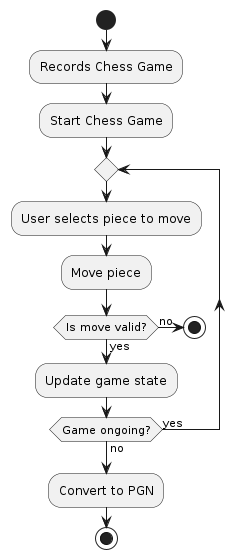
\includegraphics[height=0.75\linewidth]{figures/uml/activity.png}
    \caption[Activity Diagram]{Activity Diagram}
    \label{fig:activity}
\end{figure}

\subsection{Wireframes}
\label{subsec:wireframe}

\subsubsection*{Tournament Overview}
\label{subsubsec:tournament-overview}

\begin{figure}[h!]
    \centering
    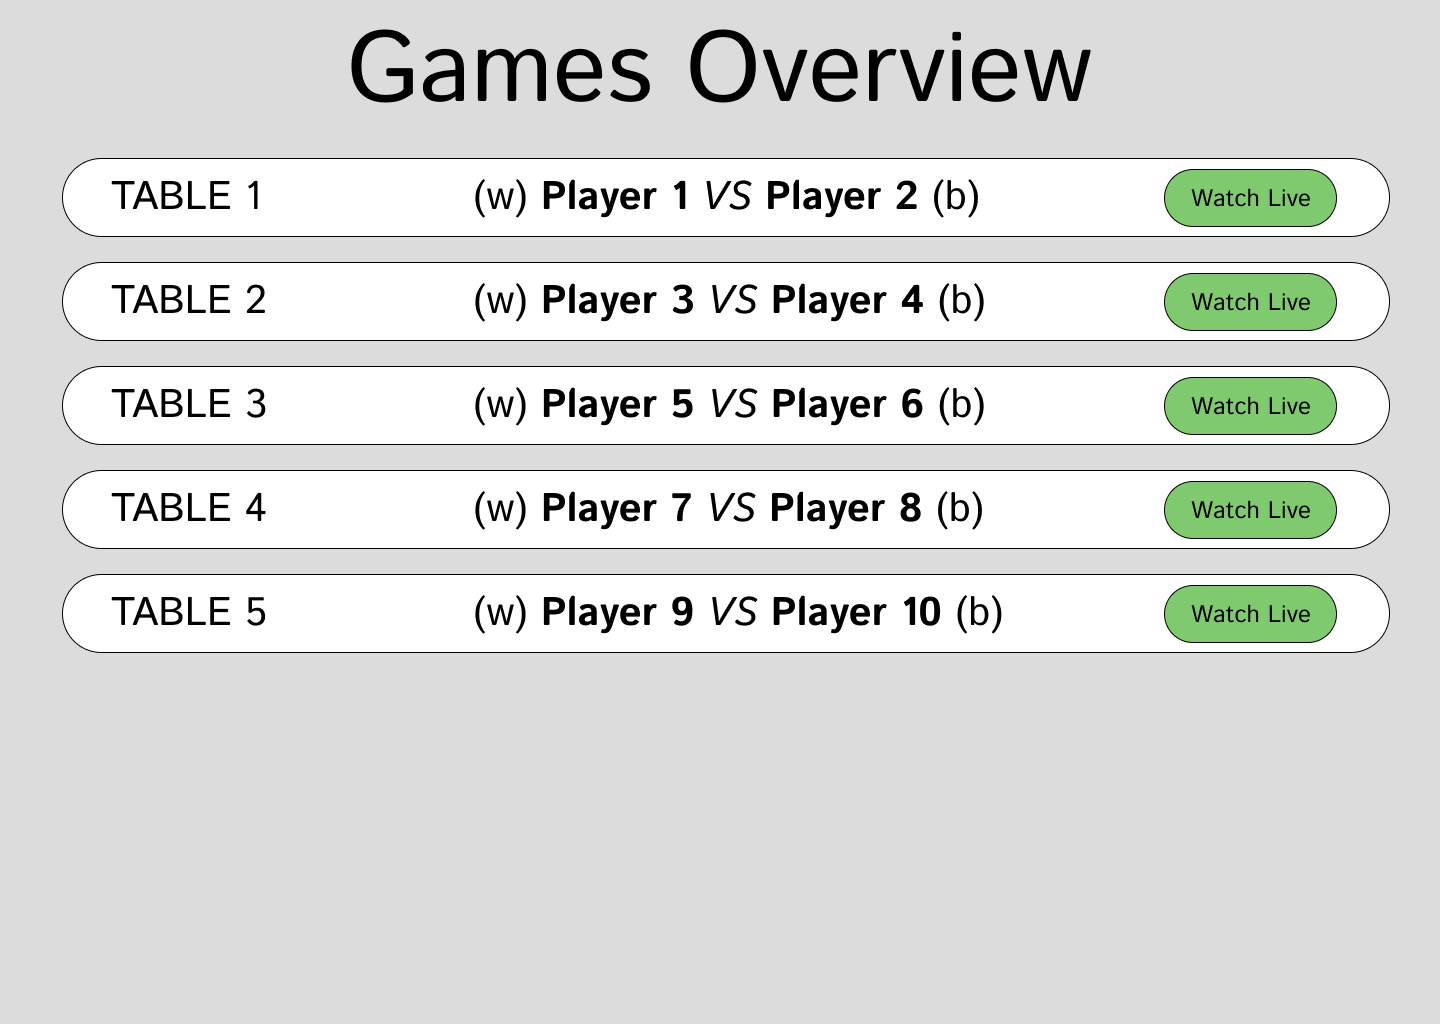
\includegraphics[width=0.75\linewidth]{figures/wireframe/overview.png}
    \caption[Games Overview Wireframe]{Wireframe of the Games Overview}
    \label{fig:app-overview}
\end{figure}

\subsubsection*{Table View}
\label{subsubsec:table-view}

\begin{figure}[h!]
    \centering
    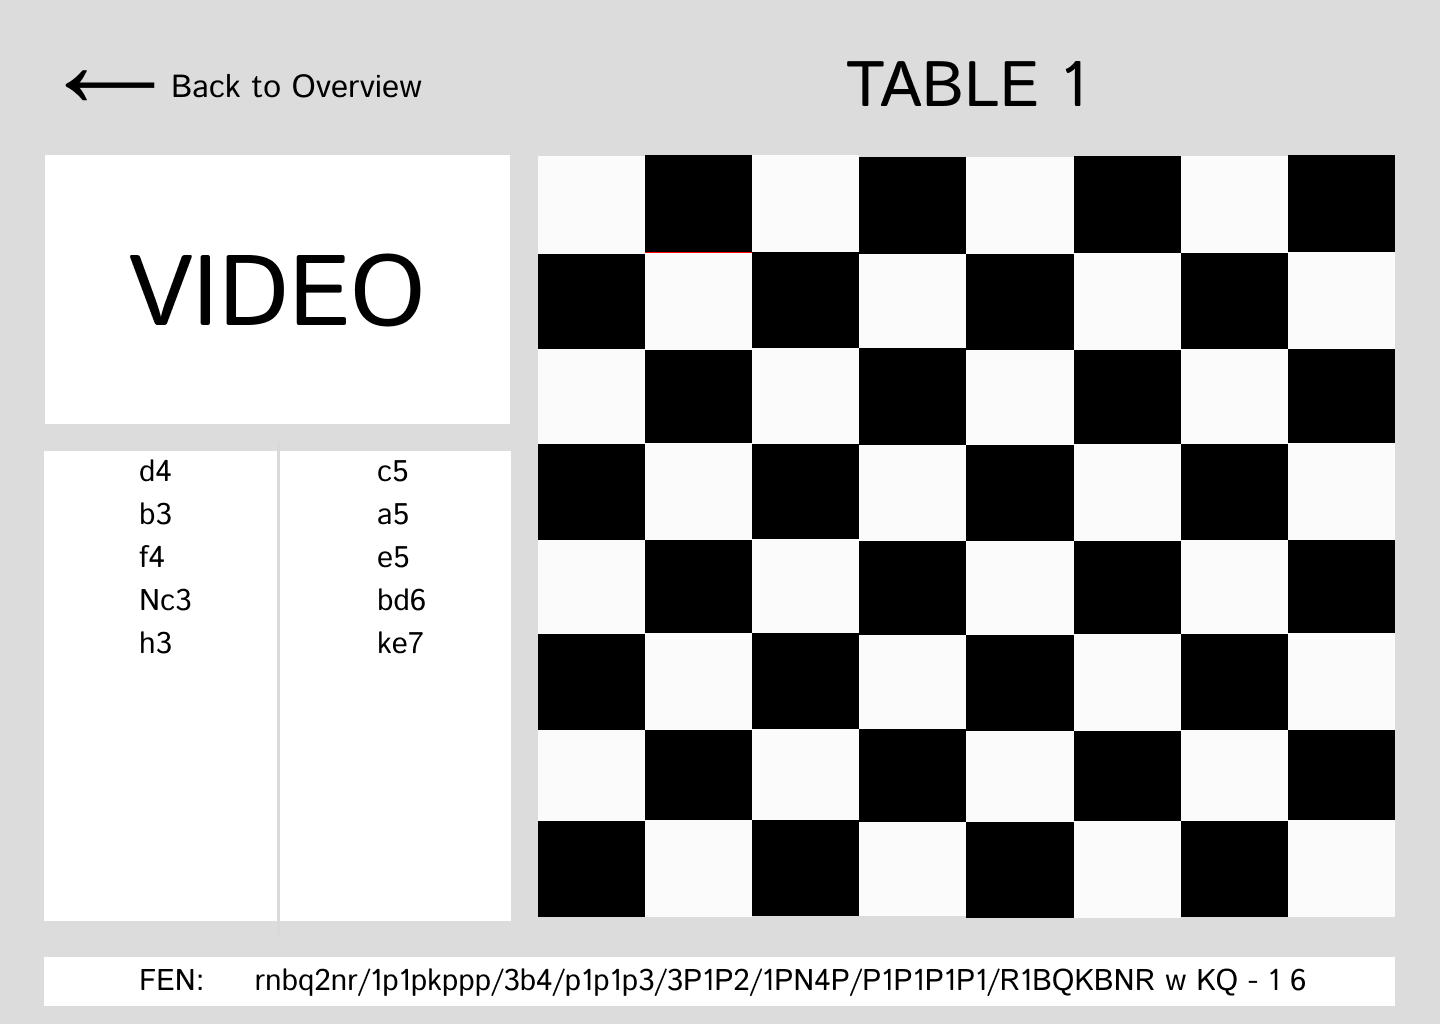
\includegraphics[width=0.75\linewidth]{figures/wireframe/table-view.png}
    \caption[Table View Wireframe]{Wireframe of the Table View of a Game on Table 1}
    \label{fig:app-table-view}
\end{figure}

\section{Tools and Platforms}
\label{sec:tools-and-platforms}

\subsection{Development Tools}
\label{subsec:development-tools}

\subsubsection*{Visual Studio Code}
\label{subsubsec:visual-studio-code}

\subsubsection*{Postman}
\label{subsubsec:postman}

\subsubsection*{Netron.app}
\label{subsubsec:natron}

\subsubsection*{Git}
\label{subsubsec:git}

\subsubsection*{ChatGPT}
\label{subsubsec:chatgpt}

\subsection{Collaboration and Design Tools}
\label{subsec:collaboration-and-design-tools}

\subsubsection*{GitHub}
\label{subsubsec:github}

\subsubsection*{Figma}
\label{subsubsec:figma}

\subsubsection*{OneDrive}
\label{subsubsec:onedrive}

\subsubsection*{Overleaf}
\label{subsubsec:overleaf}

\section{Technology Stack}
\label{sec:technology-stack}

\subsection{Backend}
\label{subsec:backend}

For the backend technology, Python is being used.

\subsubsection*{Python Libraries}
\label{subsubsec:python-libraries}

\begin{itemize}
    \item \texttt{chess} is a library for Python, with move generation, move validation, and support for common formats. \cite{python:chess}
    
    \item \texttt{FastAPI} is a modern and fast web framework for building \Glspl{api} with Python. \cite{python:fastapi}
    
    \item \texttt{numpy} is a fundamental package for scientific computing in Python. \cite{python:numpy}
    
    \item \texttt{onnxruntime}, \texttt{onnxruntime-gpu} assists in model serialization and interface with ORT. \cite{python:onnx}
    
    \item \texttt{opencv-python}, \texttt{opencv-contrib-python}, \texttt{opencv-python-headless} is used to solve computer vision problems. \cite{python:opencv}
    
    \item \texttt{requests} allows to send HTTP requests easily. \cite{python:requests}
    
    \item \texttt{scipy} is a fundamental package for algorithms for scientific computing in python. \cite{python:scipy}
    
    \item \texttt{tensorflow}, \texttt{tensorflow-intel} makes it easy to create \gls{ml} models that can run in any environment. \cite{python:tensorflow}
\end{itemize}

\subsection{Frontend}

For the frontend technology, TypeScript is being used. As discussed in \ref{subsec:type-safety}.

\subsubsection*{TypeScript Libraries}

\begin{itemize}
    \item \texttt{Vite} is a fast frontend build tool of web applications. \cite{ts:vite}
    
    \item \texttt{React} builds user interfaces out of individual pieces called components. \cite{ts:react}
    
    \item \texttt{@vitejs/plugin-react-swc} Speeds up the Vite development server. \cite{ts:swc}
    
    \item \texttt{chess.ts} a Typescript chess library for chess move generation/validation, piece placement/movement, and check/checkmate/draw detection \cite{ts:chess}
    
    \item \texttt{react-dom} serves as the entry point to the DOM and server renderers for React. \cite{ts:react-dom}
\end{itemize}